\section{Uncertainty prescription}
\label{sec:uncertainties}

The matrix method predicts $N(\mathbf{c})=\sum_i w_i(\mathbf{c})\,N_i$, so the
statistical error of the basis templates propagates with the same weights,
\begin{equation}
\sigma^2_\mathrm{interp}(\mathbf{c}) \;=\; \sum_i w_i(\mathbf{c})^2\,\sigma_i^2 \;,
\label{eq:sigmainterp}
\end{equation}
evaluated independently in every bin. The equation separates into two factors with
different owners: the weights are a property of the basis, published once and the same
in every bin, and the $\sigma_i$ are a property of whichever templates the weights are
applied to. The band is therefore wide where the templates are thin and narrow where
they are populated, which a prescription built from the total rate cannot reproduce.

The size of the band along a coupling scan depends on the templates it is propagated
through, and so on the selection; Sec.~\ref{sec:validation_realistic_band} measures it
for two real selections. For the inclusive cross section it is largest where the yield
is smallest: $0.2\mbox{--}5.8\%$ along $c_\PH$, peaking at the cancellation near
$c_\PH\simeq-3$ where the cross section falls to $13$~fb, and $0.3\mbox{--}0.7\%$ along
$c_{\PH\mathrm{kin}}$. All nine scans pass through $0.50\%$ at the SM and stay below
$1.5\%$ except $c_\PH$ and $c_{\PH G}$, which reach $5.8\%$ and $5.1\%$; the rest are in
App.~\ref{sec:appendix_performance}. The relative band grows as the rate falls, the
absolute error being set by the templates and not by the point predicted. The two scans
differ by almost an order of magnitude in their worst case despite minima of comparable
depth, which is a property of the basis: $c_{\PH\mathrm{kin}}$ is covered by more basis
points at the relevant values, so the interpolation reaches it with smaller weights.

The band is calibrated against the scatter observed along a scan, which is the direction
a fit moves in. For every generated sample on a line through the grid, the median
absolute residual over bins is compared with the median that pure statistics would give,
$0.674\sqrt{\sigma^2_\mathrm{interp}+\sigma^2_\mathrm{stat}}$; a correctly sized band
puts the ratio at one. Averaged over the $c_\PH$--$c_{\PQt\PH}$ plane the ratio is
$0.74$, and the fraction of bins whose pull is within one standard deviation is $0.72$
against the $0.683$ of a standard normal; along the individual scans of that plane it
stays between $0.6$ and $0.9$ with no trend in one region or another. Four further
planes give ratios of $0.65$ to $0.88$ and coverages of $0.67$ to $0.76$, collected in
Tab.~\ref{tab:unc_calibration}. The band therefore covers the observed scatter, by some
$25\%$ conservatively.

Two limitations are inherited from the inputs. The $\sigma_i$ are estimated from the
event count and the negative-weight fraction of each sample, because the sample set does
not record per-bin sums of squared weights; the per-bin estimate is supported by the
pull being close to normal, while the same quantity built from the total rate is about
six times wider than the observed residual and must not be used. The second is specific
to the scans of this section: the basis templates are themselves samples of the grid the
reweighting coefficients were fitted to, so adding the interpolation uncertainty to the
uncertainty of those coefficients double counts. It amounts to forty samples of some
four thousand, with a coefficient term well below the interpolation one, and it does not
arise in the case an analysis faces, where the templates are built from its own events
and the coefficients come from the grid.

What does arise there is a correlation between templates built from the same events.
Eq.~\eqref{eq:sigmainterp} treats the $\sigma_i$ as independent, which is exact where
the basis templates are separately generated samples --- the case for every number
quoted in this section and for the calibration above --- and not where they are produced
by reweighting one set of events, as those of
Sec.~\ref{sec:validation_realistic_band} are. The exact variance is a quadratic form in
the same weights,
\begin{equation}
  \sigma^2_\mathrm{MM}(\mathbf{c}) = w(\mathbf{c})^{T} S\, w(\mathbf{c}),
  \qquad
  S_{ik} = \sum_s \alpha_s(i)\,\alpha_s(k) \sum_{e \in s} \omega_i(e)\,\omega_k(e),
  \label{eq:sigmaMMcov}
\end{equation}
evaluated in each bin, with $\omega_i(e)$ the weight that takes event $e$ to basis point
$i$ and $\alpha_s(i)$ the inverse-variance weight with which input sample $s$ enters
template $i$ in that bin. Its diagonal is the error each template carries on its own, so
Eq.~\eqref{eq:sigmainterp} is the case $S$ diagonal.

The two forms differ by factors rather than by percents. Measured on the \HHbbbb templates with
$S$ built per \mHH bin, they agree at a basis point, where the weight vector is a unit
vector, and depart from one another elsewhere: integrated over \mHH the independent form
is between $0.7$ and $9$ times the exact one over the points tested, and bin by bin
between $0.6$ and about $30$, mostly above it, the departure growing with
$\sum_i|w_i|$. The templates are reweightings of the same events, so their fluctuations
cancel in the morphed sum where the independent form adds them in quadrature. An
analysis whose templates come from a common set of events should therefore use
Eq.~\eqref{eq:sigmaMMcov}, which costs one pass over its own events with every basis
point's weight, or propagate the uncertainty through the reweighting evaluated directly
at the point in question, which carries the correlation automatically.

Fig.~\ref{fig:unc_band_by_bin} resolves the band into the \mHH bins it is computed from,
at four points of the $c_\PH$ scan. In every bin the weights are the same; what differs
is how many events the basis templates have there. The band is below $1\%$ near
threshold, where the templates are well populated, and reaches tens to hundreds of
percent above $1.5$~TeV, where they hold few events. The curve at $c_\PH=-3$ is large at
low mass as well: there the prediction is a difference of comparable contributions, so a
small absolute error on the templates is a large relative error on what survives.

\begin{figure}[htbp]
    \centering
    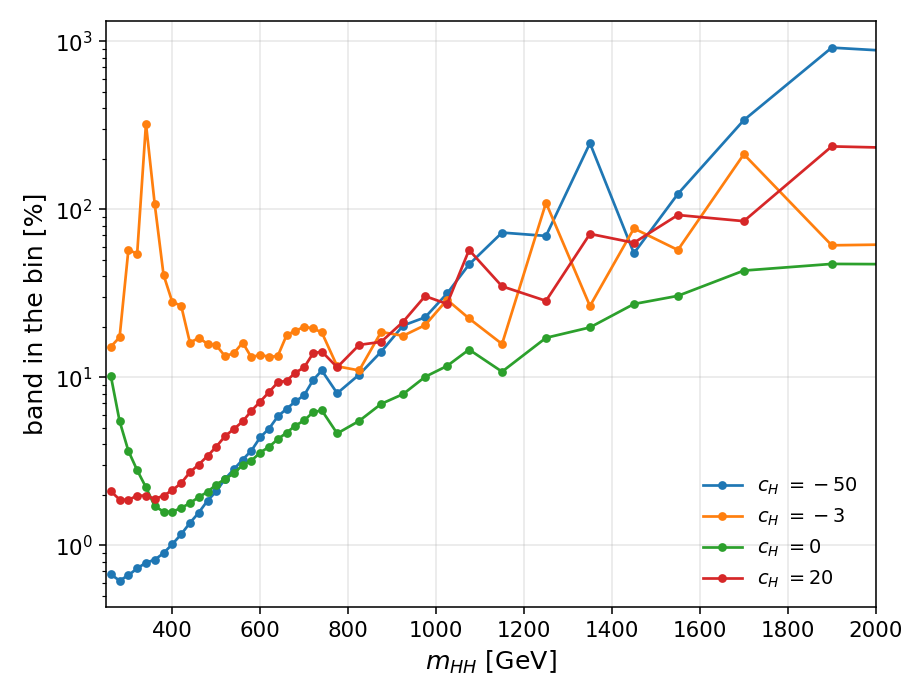
\includegraphics[width=0.49\textwidth]
        {figures/basis_optimization/unc_band_by_bin.png}%
    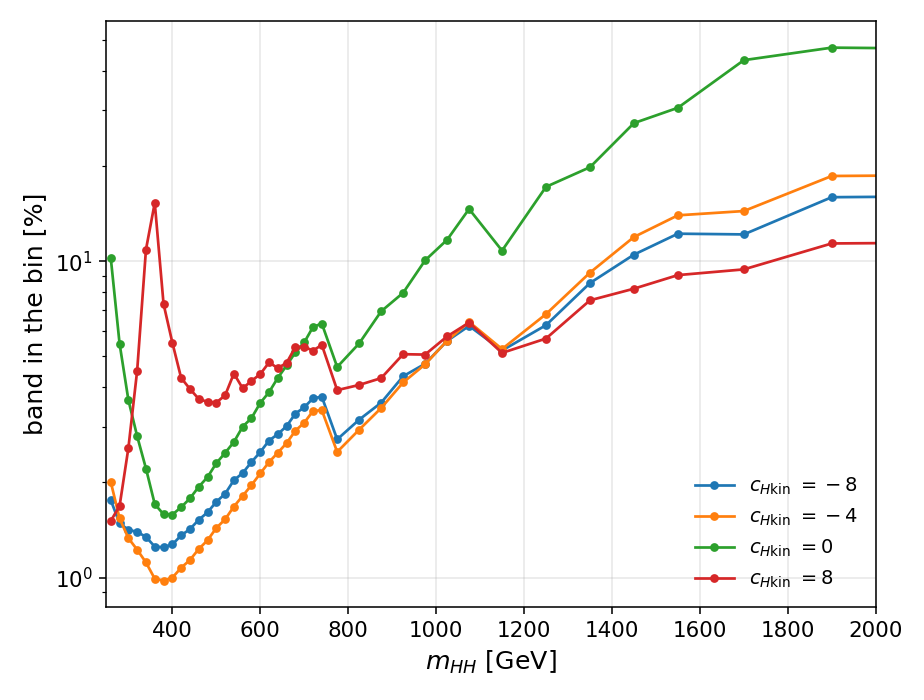
\includegraphics[width=0.49\textwidth]
        {figures/basis_optimization/unc_band_by_bin_cHkin.png}
    \caption{Interpolation uncertainty of Eq.~\eqref{eq:sigmainterp} in each
    \mHH bin, as a fraction of the predicted content of that bin, at four
    values of $c_\PH$ (left) and of $c_{\PH\mathrm{kin}}$ (right), the other
    eight coefficients at zero in each case.}
    \label{fig:unc_band_by_bin}
\end{figure}

Integrated over \mHH the same band is a few percent, which is why the prescription has
to be differential. The bins with the largest relative uncertainty carry almost none of
the yield, so summing over bins lets the well-populated low-mass bins dominate and
the tail contribute little. A number quoted from the total alone would be those few
percent and would not record that part of the spectrum is predicted only to within a
factor, which is what an analysis fitting the tail needs.

That separation is measured in Sec.~\ref{sec:validation_realistic_band}, where the
weights published here are applied to the templates of two different $\HH\to\bbbar\bbbar$ selections and
give two bands differing by a factor of five to ten, with nothing about the effective
field theory re-derived in between. The prescription transfers; the numbers quoted in
this section do not.

In a fit the band need not be evaluated at all. Since
$N_j(\mathbf{c})=\sum_i w_i(\mathbf{c})N_{ij}$, giving each basis template its own
statistical uncertainty and letting the fit recompute the sum with the varied templates
reproduces Eq.~\eqref{eq:sigmainterp}, carries its dependence on $\mathbf{c}$, and keeps
the cancellations between weights of opposite sign. Where the forty templates are
themselves the inputs the model morphs, an automatic treatment of the template
statistics already does this. Precomputing the band at one coupling point and quoting it
as a fixed shape uncertainty is adequate only near the SM: over the generated ranges the
band varies by an order of magnitude.

The uncertainty of the reweighting coefficients the templates were made with is a
separate term and stays one nuisance. It is a single source, correlated across templates
and bins, so a coherent shift of it partly cancels in the weighted sum where the
independent statistical errors add in quadrature, and treating it as one nuisance per
template would overstate it. It is the larger of the two in the resolved selection for
every coefficient of Fig.~\ref{fig:acc_4b}, so a prediction carrying only the template
statistics understates its total modelling uncertainty by a factor of a few. The two are
combined as $\sigma_\mathrm{mod}^2=\sigma_\mathrm{MM}^2+\sigma_\mathrm{ELR}^2$ and are
given separately per selection in Tab.~\ref{tab:unc_components}.

A card built this way carries three terms that do not overlap. The Monte Carlo
statistical uncertainty of the background enters through the Barlow--Beeston-lite
treatment of Combine, which leaves the signal processes out; that of the morphed signal
enters through one nuisance parameter per channel of size
$\sigma_\mathrm{MM}(\mathbf{c})/N(\mathbf{c})$, computed from the covariance of the basis
templates and following the coefficients as they move; and the reweighting coefficients enter as the single
correlated nuisance parameter described above.

Beyond the interpolation, the \ggHH prediction carries its own theory uncertainty, and
the nine-coefficient model inherits it from the $\kappa$ models unchanged: the QCD scale
and top-mass envelope of the non-resonant \ggHH cross section, applied as a single
nuisance scaling every \ggHH sample alike. The envelope is tabulated against
$\kappa_\lambda$, so the model evaluates it at the $\kappa_\lambda$ obtained from the
Wilson coefficients by the naive translation of Eq.~\eqref{eq:naivetranslation}, which at
$\Lambda=1$~TeV reads $\kappa_\lambda = 1 - 0.469\,c_\PH + 0.182\,c_{\PH\mathrm{kin}}$.
Being a common factor of all \ggHH samples it does not interact with the morphing: it
multiplies the prediction after the templates are combined, and is unaffected by the
restriction of Sec.~\ref{sec:slice_models}, since the templates left out there have a
vanishing morphing weight.

Two properties of that prescription follow. The envelope is not re-expressed as
a function of the Wilson coefficients: it is the $\kappa_\lambda$ envelope evaluated at
the translated point, so it remains the same object the $\kappa$ models use and follows
any update to it. Writing it out in $c_\PH$ instead would fix $\Lambda$, since the
translation carries $v^2/\Lambda^2$, and an analysis at a different $\Lambda$ would
silently get the wrong uncertainty. The envelope also covers only the trilinear
direction: it was built by varying $\kappa_\lambda$, so the part of
$c_{\PH\mathrm{kin}}$ that rescales the top Yukawa, and the scale dependence introduced
by the operators with no $\kappa_\lambda$ image, are not included in it.
